\documentclass[class=minimal,border=0pt, 11pt]{standalone}
\usepackage{mathpazo}
\usepackage{xcolor}
\usepackage{amsmath, amsfonts, mathtools, amssymb, amsthm} 
\usepackage{tikz, pgfplots}
\pgfplotsset{compat=1.8}
\DeclareMathOperator{\parab}{par}
\definecolor{darkgreen}{rgb}{0.0 0.5 0.0}
\definecolor{whitegreen}{rgb}{0.0 0.75 0.0}
\definecolor{whiteblue}{rgb}{0.0 0.0 1.2}
\definecolor{darkred}{rgb}{0.8 0.0 0.0}
\def\samplepar{10}
\def\sampleatn{30}
\def\samplesamp{35}
\newcommand{\xb}{\mathbf{x}}
\begin{document} 

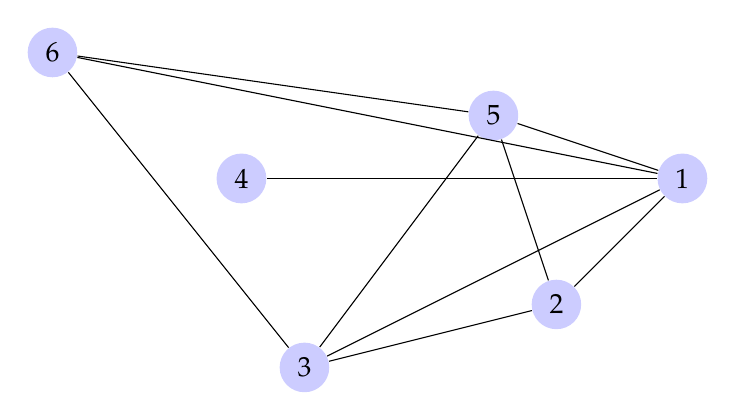
\begin{tikzpicture}
  [scale=.8,auto=left,every node/.style={circle,fill=blue!20}]
  \node (n6) at (1,10) {6};
  \node (n4) at (4,8)  {4};
  \node (n5) at (8,9)  {5};
  \node (n1) at (11,8) {1};
  \node (n2) at (9,6)  {2};
  \node (n3) at (5,5)  {3};
  \foreach \from/\to in {n1/n2,n1/n3,n1/n4,n1/n5,n1/n6,n2/n3,n2/n5,n3/n5,n3/n6,n5/n6}
    \draw (\from) -- (\to);
\end{tikzpicture}

\end{document} 